\documentclass[reqno,a4paper,12pt]{amsart}

\usepackage{amsmath,amssymb,amsthm,geometry,xcolor,soul,graphicx}
\usepackage{titlesec}
\usepackage{enumerate}
\usepackage{lipsum}
\usepackage{listings}
\RequirePackage[most]{tcolorbox}
%\usepackage{braket}
%\usepackage{esint} %$\varoiint$ (带圈的二重积分)
%\usepackage[colorlinks,linkcolor=red]{hyperref} %\url{}超链接
\usepackage{xeCJK}
\setCJKmainfont{Kai}
\geometry{left=0.7in, right=0.7in, top=1in, bottom=1in}

\renewcommand{\baselinestretch}{1.3}

\title{固体物理第五次作业}
\author{董建宇 ~~ 2019511017}

\begin{document}

\maketitle
\titleformat{\section}[hang]{\small}{\thesection}{0.8em}{}{}
\titleformat{\subsection}[hang]{\small}{\thesubsection}{0.8em}{}{}

\section{\textbf{(8.1) Potentials Between Atoms}}
%\begin{enumerate}[(a)]
As a model of thermal expansion, we study the distance between two nearest-neighbor atoms in an anharmonic potential that looks roughly like this 
\begin{center}
	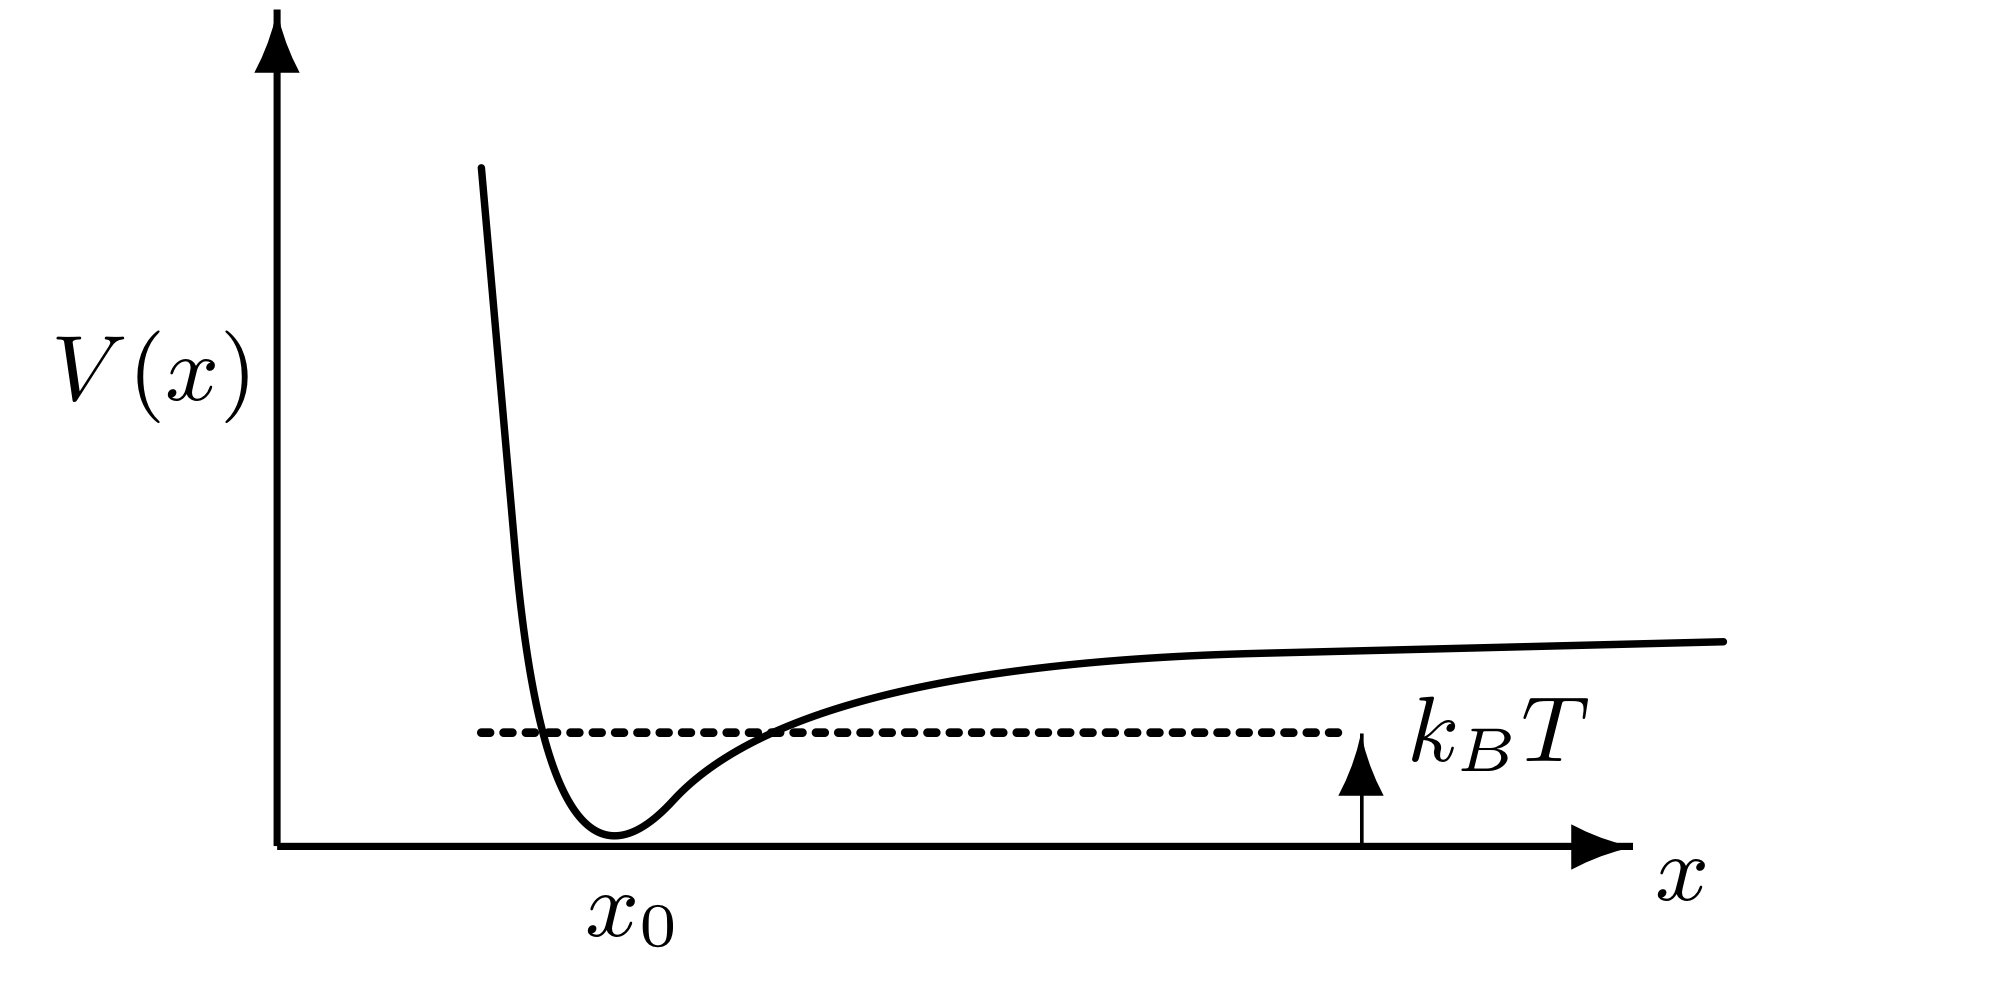
\includegraphics[scale = 0.25]{8-1.jpeg}
\end{center} 
where $x$ is the distance between the two neighboring atoms. This potential can be expanded around its minimum as 
\[
	V(x) = \frac{\kappa}{2}(x-x_0)^2 - \frac{\kappa_3}{3!}(x-x_0)^3 + \dots
\]
where the minimum is at position $x_0$ and $\kappa_3>0$. For small energies, we can truncate the series at the cubic term. (Note that we are defining the energy at the bottom of the well to be zero here.) \\
A very accurate approximate form for interatomic potentials (particularly for inert atoms such as helium or argon) is given by the so-call Lennard-Jones potential 
\[
	V(x) = 4\epsilon \left[ \left(\frac{\sigma}{x}\right)^{12} - \left( \frac{\sigma}{x} \right)^6 \right] + \epsilon
\]
where $\epsilon$ and $\sigma$ are constants that depend on the particular atoms we are considering. \\
$\triangleright$ What is the meaning of the exponent 6 in the second term of this expression (i.e., why is the exponent necessarily chosen to be 6). 
\begin{tcolorbox}[breakable, colback = black!5!white, colframe = black]
	当原子间距离增大时,两原子的互相吸引力可近似为两个偶极子的吸引,能量反比于$r^{-6}$,则当$x >> x_0$($x_0$为平衡位置)时,势能函数以$-x^{-6}$趋势增加,则第二项指数为$6$。
\end{tcolorbox}

$\triangleright$ By expanding Eq. 8.5 around its minimum, and comparing to Eq. 8.4, calculate the values of the coefficients $x_0$, $\kappa$ and $\kappa_3$ for the Lennard-Jones potential in therm of the constants $\epsilon$ and $\sigma$. We will need these results in Exercise 8.3
\begin{tcolorbox}[breakable, colback = black!5!white, colframe = black]
一阶导数在$x_0$处的值为0;二阶导数在$x_0$处的值为$\kappa$;三阶导数在$x_0$处的值为$-\kappa_3$,则有:
\[
	4\epsilon\left( -12\frac{\sigma^{12}}{x_0^{13}} + 6\frac{\sigma^6}{x_0^7} \right) = 0.
\]
\[
	4\epsilon\left( 156\frac{\sigma^{12}}{x_0^{14}} - 42\frac{\sigma^6}{x_0^8} \right) = \kappa.
\]
\[
	4\epsilon\left( -2184\frac{\sigma^{12}}{x_0^{15}} + 336\frac{\sigma^6}{x_0^9} \right) = -\kappa_3
\]
可以解得:
\[
	x_0 = \sqrt[6]{2}\sigma, ~~ \kappa = \frac{72\epsilon}{\sqrt[3]{2}\sigma^2}, ~~ \kappa_3 = \frac{1512\epsilon}{\sqrt{2}\sigma^3}.
\]
\end{tcolorbox}


\section{\textbf{9.1 Classical Normal Modes to Quantum Eigenstates}}
In Section 9.3 we stated without proof that a classical normal mode becomes a quantum eigenstate. Here we prove this fact for a simple diatomic molecule in a potential well (see Exercise 2.7 for a more difficult case, and see also Exercise 9.7 where this principle is proven in more generally). \\
Consider two particles, each of mass $m$ in one dimension, connected by a spring ($K$), at the bottom of a potential well (with spring constant $k$). We write the potential energy as 
\[
	U = \frac{k}{2}(x_1^2+x_2^2) + \frac{K}{2}(x_1-x_2)^2
\]

$\triangleright$ Write the classical equations of motion. 
\begin{tcolorbox}[breakable, colback = black!5!white, colframe = black]
处在$x_1$处粒子受力为:$-\frac{\partial U}{\partial x_1}$,处在$x_2$处粒子受力为:$-\frac{\partial U}{\partial x_2}$。则经典动力学方程为:
\[
	m\ddot{x}_1 = -k x_1 - K(x_1-x_2),
\]
\[
	m\ddot{x}_2 = -k x_2 + K(x_1-x_2).
\]
\end{tcolorbox}
$\triangleright$ Transform into relative $x_{rel} = (x_1-x_2)$ and center of mass $x_{cm} = (x_1+x_2)/2$ coordinates.
\begin{tcolorbox}[breakable, colback = black!5!white, colframe = black]
令$x_{rel} = x_1 - x_2$,$x_{cm} = (x_1+x_2)/2$可得:
\[
	x_1 = x_{cm} + \frac{1}{2}x_{rel}, ~~ x_2 = x_{cm} - \frac{1}{2}x_{rel}.
\]
则有:
\[
	m\left( \ddot{x}_{cm} + \frac{1}{2}\ddot{x}_{rel} \right) = -k\left( x_{cm} + \frac{1}{2}x_{rel} \right) - Kx_{rel}.
\]
\[
	m\left( \ddot{x}_{cm} - \frac{1}{2}\ddot{x}_{rel} \right) = -k\left( x_{cm} - \frac{1}{2}x_{rel} \right) + Kx_{rel}
\]
两式相加得:
\[
	m\ddot{x}_{cm} = -kx_{cm}.
\]
两式相减得:
\[
	m\ddot{x}_{rel} = -k x_{rel} - 2K x_{rel}.
\]
\end{tcolorbox}
(a) Show that in these transformed coordinates, the system decouples, thus showing that the two normal modes have frequencies 
\begin{align*}
	\omega_{cm} &= \sqrt{k/m} \\
	\omega_{rel} &= \sqrt{(k+2K/m)}.
\end{align*}
Note that since there are two initial degrees of freedom, there are two normal modes. \\
Now consider the quantum-mechanical version of the same problem. The Hamiltonian is 
\[
	H = \frac{p_1^2}{2m} + \frac{p_2^2}{2m} + U(x_1,x_2)
\]
$\triangleright$ Again transform into relative and center of mass coordinates. \\
Define the corresponding momenta $p_{rel} = (p_1-p_2)/2$ and $p_{cm} = (p_1+p_2)$.
\begin{tcolorbox}[breakable, colback = black!5!white, colframe = black]
由上述$\ddot{x}_{cm}$和$\ddot{x}_{rel}$满足的方程变形可得:
\begin{align*}
	\ddot{x}_{cm} &= -\frac{k}{m}x_{cm} \\
	\ddot{x}_{rel} &= -\frac{k+2K}{m}x_{rel}.
\end{align*}
则两正则坐标对应模式频率为:
\[
	\omega_{cm} = \sqrt{k/m}, ~~ \omega_{rel} = \sqrt{(k+2K)/m}.
\]
由$p_{rel} = (p_1-p_2)/2$以及$p_{cm} = p_1+p_2$可知:
\[
	p_1 = p_{rel} +\frac{p_{cm}}{2}, ~~ p_2 = -p_{rel} + \frac{p_{cm}}{2}.
\]
则Hamiltonian量为:
\[
	H = \frac{p_{rel}^2}{m} + \frac{p_{cm}^2}{4m} + k\left(x_{cm}^2 + \frac{1}{4}x_{rel}^2 \right) + \frac{K}{2}x_{rel}^2.
\]
\end{tcolorbox}

(b) Show that $[p_\alpha, x_\gamma] = -i\hbar\delta_{\alpha,\gamma}$ where $\alpha$ and $\gamma$ take the values $cm$ or $rel$.
\begin{tcolorbox}[breakable, colback = black!5!white, colframe = black]
由$[x_i, p_j] = i\hbar\delta_{i,j}$,其中$i,j = 1,2$。则可以计算:
\begin{align*}
	[p_{rel}, x_{rel}] &= \frac{1}{2}([p_1,x_1] - [p_1,x_2] - [p_2,x_1] + [p_2,x_2]) = \frac{1}{2}(-i\hbar-0-0-i\hbar) = -i\hbar. \\
	[p_{rel}, x_{cm}] &= \frac{1}{4}([p_1,x_1] + [p_1,x_2] - [p_2,x_1] - [p_2,x_2]) = \frac{1}{4}(-i\hbar + 0 - 0 + i\hbar) = 0. \\
	[p_{cm}, x_{rel}] &= [p_1,x_1] - [p_1,x_2] + [p_2,x_1] - [p_2,x_2] = -i\hbar - 0 + 0 + i\hbar = 0. \\
	[p_{cm}, x_{cm}] &= \frac{1}{2}([p_1,x_1] + [p_1,x_2] + [p_2,x_1] + [p_2,x_2]) = \frac{1}{2}(-i\hbar+0+0-i\hbar) = -i\hbar.
\end{align*}
综上所述,有:
\[
	[p_\alpha, x_\gamma] = -i\hbar\delta_{\alpha,\gamma}
\]
其中$\alpha$与$\gamma$从$cm$和$rel$中取值。
\end{tcolorbox}

(c) In terms of these new coordinates show that the Hamiltonian decouples into two independent harmonic oscillators with the same eigenfrequencies $\omega_{cm}$ and $\omega_{rel}$. Conclude that the spectrum of this system is 
\[
	E_{n_{rel}, n_{cm}} = \hbar\omega_{rel} (n_{rel} + \frac{1}{2}) + \hbar\omega_{cm}(n_{cm} + \frac{1}{2})
\]
where $n_{cm}$ and $n_{rel}$ are non-negative integers.
\begin{tcolorbox}[breakable, colback = black!5!white, colframe = black]
Hamiltonian 算符可以写为:
\[
	H = \frac{p_{rel}^2}{2(m/2)} + \frac{1}{2}(K+k/2)x_{rel}^2 + \frac{p_{cm}^2}{2(2m)} + \frac{1}{2}(2k) x_{cm}^2 = H_1 + H_2.
\]
其中
\[
	H_1 = \frac{p_{rel}^2}{2(m/2)} + \frac{1}{2}\frac{m}{2}\omega_{rel}^2x_{rel}^2, ~~ H_2 = \frac{p_{cm}^2}{2(2m)} + \frac{1}{2}(2m)\omega_{cm}^2x_{cm}^2.
\]
则有$H_1$的本征值为:$E_1 = \hbar\omega_{rel}(n_{rel}+1/2)$,$H_2$的本征值为:$E_2 = \hbar\omega_{cm}(n_{cm}+1/2)$。则Hamiltonian本征值为:
\[
	E_{n_{rel}, n_{cm}} =E_1 + E_2 = \hbar\omega_{rel} (n_{rel} + \frac{1}{2}) + \hbar\omega_{cm}(n_{cm} + \frac{1}{2}).
\]
其中$n_{rel}$,$n_{cm}$为非负整数。
\end{tcolorbox}

(d) At temperature T what is the expectation of the energy of this system?
\begin{tcolorbox}[breakable, colback = black!5!white, colframe = black]
对于处在温度T下的简谐振子,能量平均值为:
\[
	\langle E_1 \rangle = \hbar\omega_{rel} \left( \frac{1}{e^{\beta\hbar\omega_{rel}} - 1} + \frac{1}{2} \right), ~~ \langle E_2 \rangle = \hbar\omega_{cm} \left( \frac{1}{e^{\beta\hbar\omega_{cm}} - 1} + \frac{1}{2} \right).
\]
则总能量平均值为:
\[
	\langle E \rangle = \hbar\omega_{rel} \left( \frac{1}{e^{\beta\hbar\omega_{rel}} - 1} + \frac{1}{2} \right) + \hbar\omega_{cm} \left( \frac{1}{e^{\beta\hbar\omega_{cm}} - 1} + \frac{1}{2} \right).
\]
其中$\beta = \frac{1}{kT}$。
\end{tcolorbox}

\section{\textbf{(9.2) Normal Modes of a One-Dimensional Monatomic Chain}}
\begin{enumerate}[(a)]
	\item $\ddagger$ Explain what is meant by "normal mode" and by "phonon". \\
	$\triangleright$ Explain briefly why phonons obey Bose statistics.
	\begin{tcolorbox}[breakable, colback = black!5!white, colframe = black]
	\textbf{Normal modes} are collective oscillations where all particles move at the same frequency. (即所有粒子以相同的频率震荡。) \\
	A \textbf{phonon} is a discrete quantum of vibration. (即声子是一个携带能量、动量的离散的量子)。 \\
	如果把声子考虑为一个粒子,则我们可以在同一个量子态中放入许多个声子,因此声子类似光子服从玻色分布。
	\end{tcolorbox}
		
	\item $\ddagger$ Derive the dispersion relation for the longitudinal oscillations of a one-dimensional mass-and-spring crystal with $N$ identical atoms of mass $m$, lattice spacing $a$, and spring constant $\kappa$ (motion of the masses is restricted to be in one dimension).
	\begin{tcolorbox}[breakable, colback = black!5!white, colframe = black]
	考虑第$n$个粒子,动力学方程为:
	\[
		m\ddot{x}_n = \kappa(x_{n+1} - x_n) - \kappa(x_n-x_{n-1}) = \kappa(x_{n+1}+x_{n-1}-2x_n).
	\]
	假设通解为:
	\[
		x_n = A e^{i\omega t-ikna}.
	\]
	则有
	\[
		-\omega^2me^{i\omega t-ikna} = \kappa e^{i\omega t}(e^{-ik(n+1)a} + e^{-ik(n-1)a} - 2e^{-ikna}).
	\]
	即
	\[
		\omega^2 = \frac{2\kappa}{m}(1-\cos(ka)).
	\]
	两侧开平方得:
	\[
		\omega = 2\sqrt{\frac{\kappa}{m}}\left\vert \sin\left( \frac{ka}{2} \right) \right\vert.
	\]
	\end{tcolorbox}

	\item $\ddagger$ Show that the mode with wavevectors $k$ has the same pattern of mass displacements as the mode with wavevectors $k+2\pi/a$. Hence show that the dispersion relation is periodic in reciprocal space ($k$-space). \\
	$\triangleright$ How many different normal modes are there.
	\begin{tcolorbox}[breakable, colback = black!5!white, colframe = black]
	\[
	Ae^{i\omega t - i(k+2\pi/a)na} = A e^{i\omega t-ikna} e^{-i2n\pi} =  A e^{i\omega t-ikna} = x_n.
	\]
	即波矢量为$k$与波矢量为$k+2\pi/a$为同一模式。即色散关系在倒空间中具有周期性。\\
	简正模式共有:
	\[
		\frac{2\pi/a}{2\pi/(Na)} = N.
	\]
	\end{tcolorbox}
	
	\item $\ddagger$ Derive the phase and group velocities and sketch them as a function of $k$. \\
	$\triangleright$ What is the sound velocity? \\
	$\triangleright$ Show that the sound velocity is also given by $v_s = \frac{1}{\sqrt{\beta\rho}}$ where $\rho$ is the chain density and $\beta$ is the compressibility.
	\begin{tcolorbox}[breakable, colback = black!5!white, colframe = black]
	相速度为:
	\[
		v_p = \frac{\omega}{k} = 2\sqrt{\frac{\kappa}{m}}\frac{1}{k} \left\vert \sin\left( \frac{ka}{2} \right) \right\vert.
	\]
	在第一布里渊区群速度为:
	\[
		v_g = \frac{\partial \omega}{\partial k} = \left\{ \begin{aligned}
		&a\sqrt{\frac{\kappa}{m}}\cos\left( \frac{ka}{2} \right) &  &0<\frac{ka}{2} < \frac{\pi}{2}\\
		&-a\sqrt{\frac{\kappa}{m}}\cos\left( \frac{ka}{2} \right) & &-\frac{\pi}{2} <\frac{ka}{2} < 0 
	\end{aligned}\right.
	\]
	取$a = 1,\kappa = m = 1$绘图如下:
	\begin{center}
		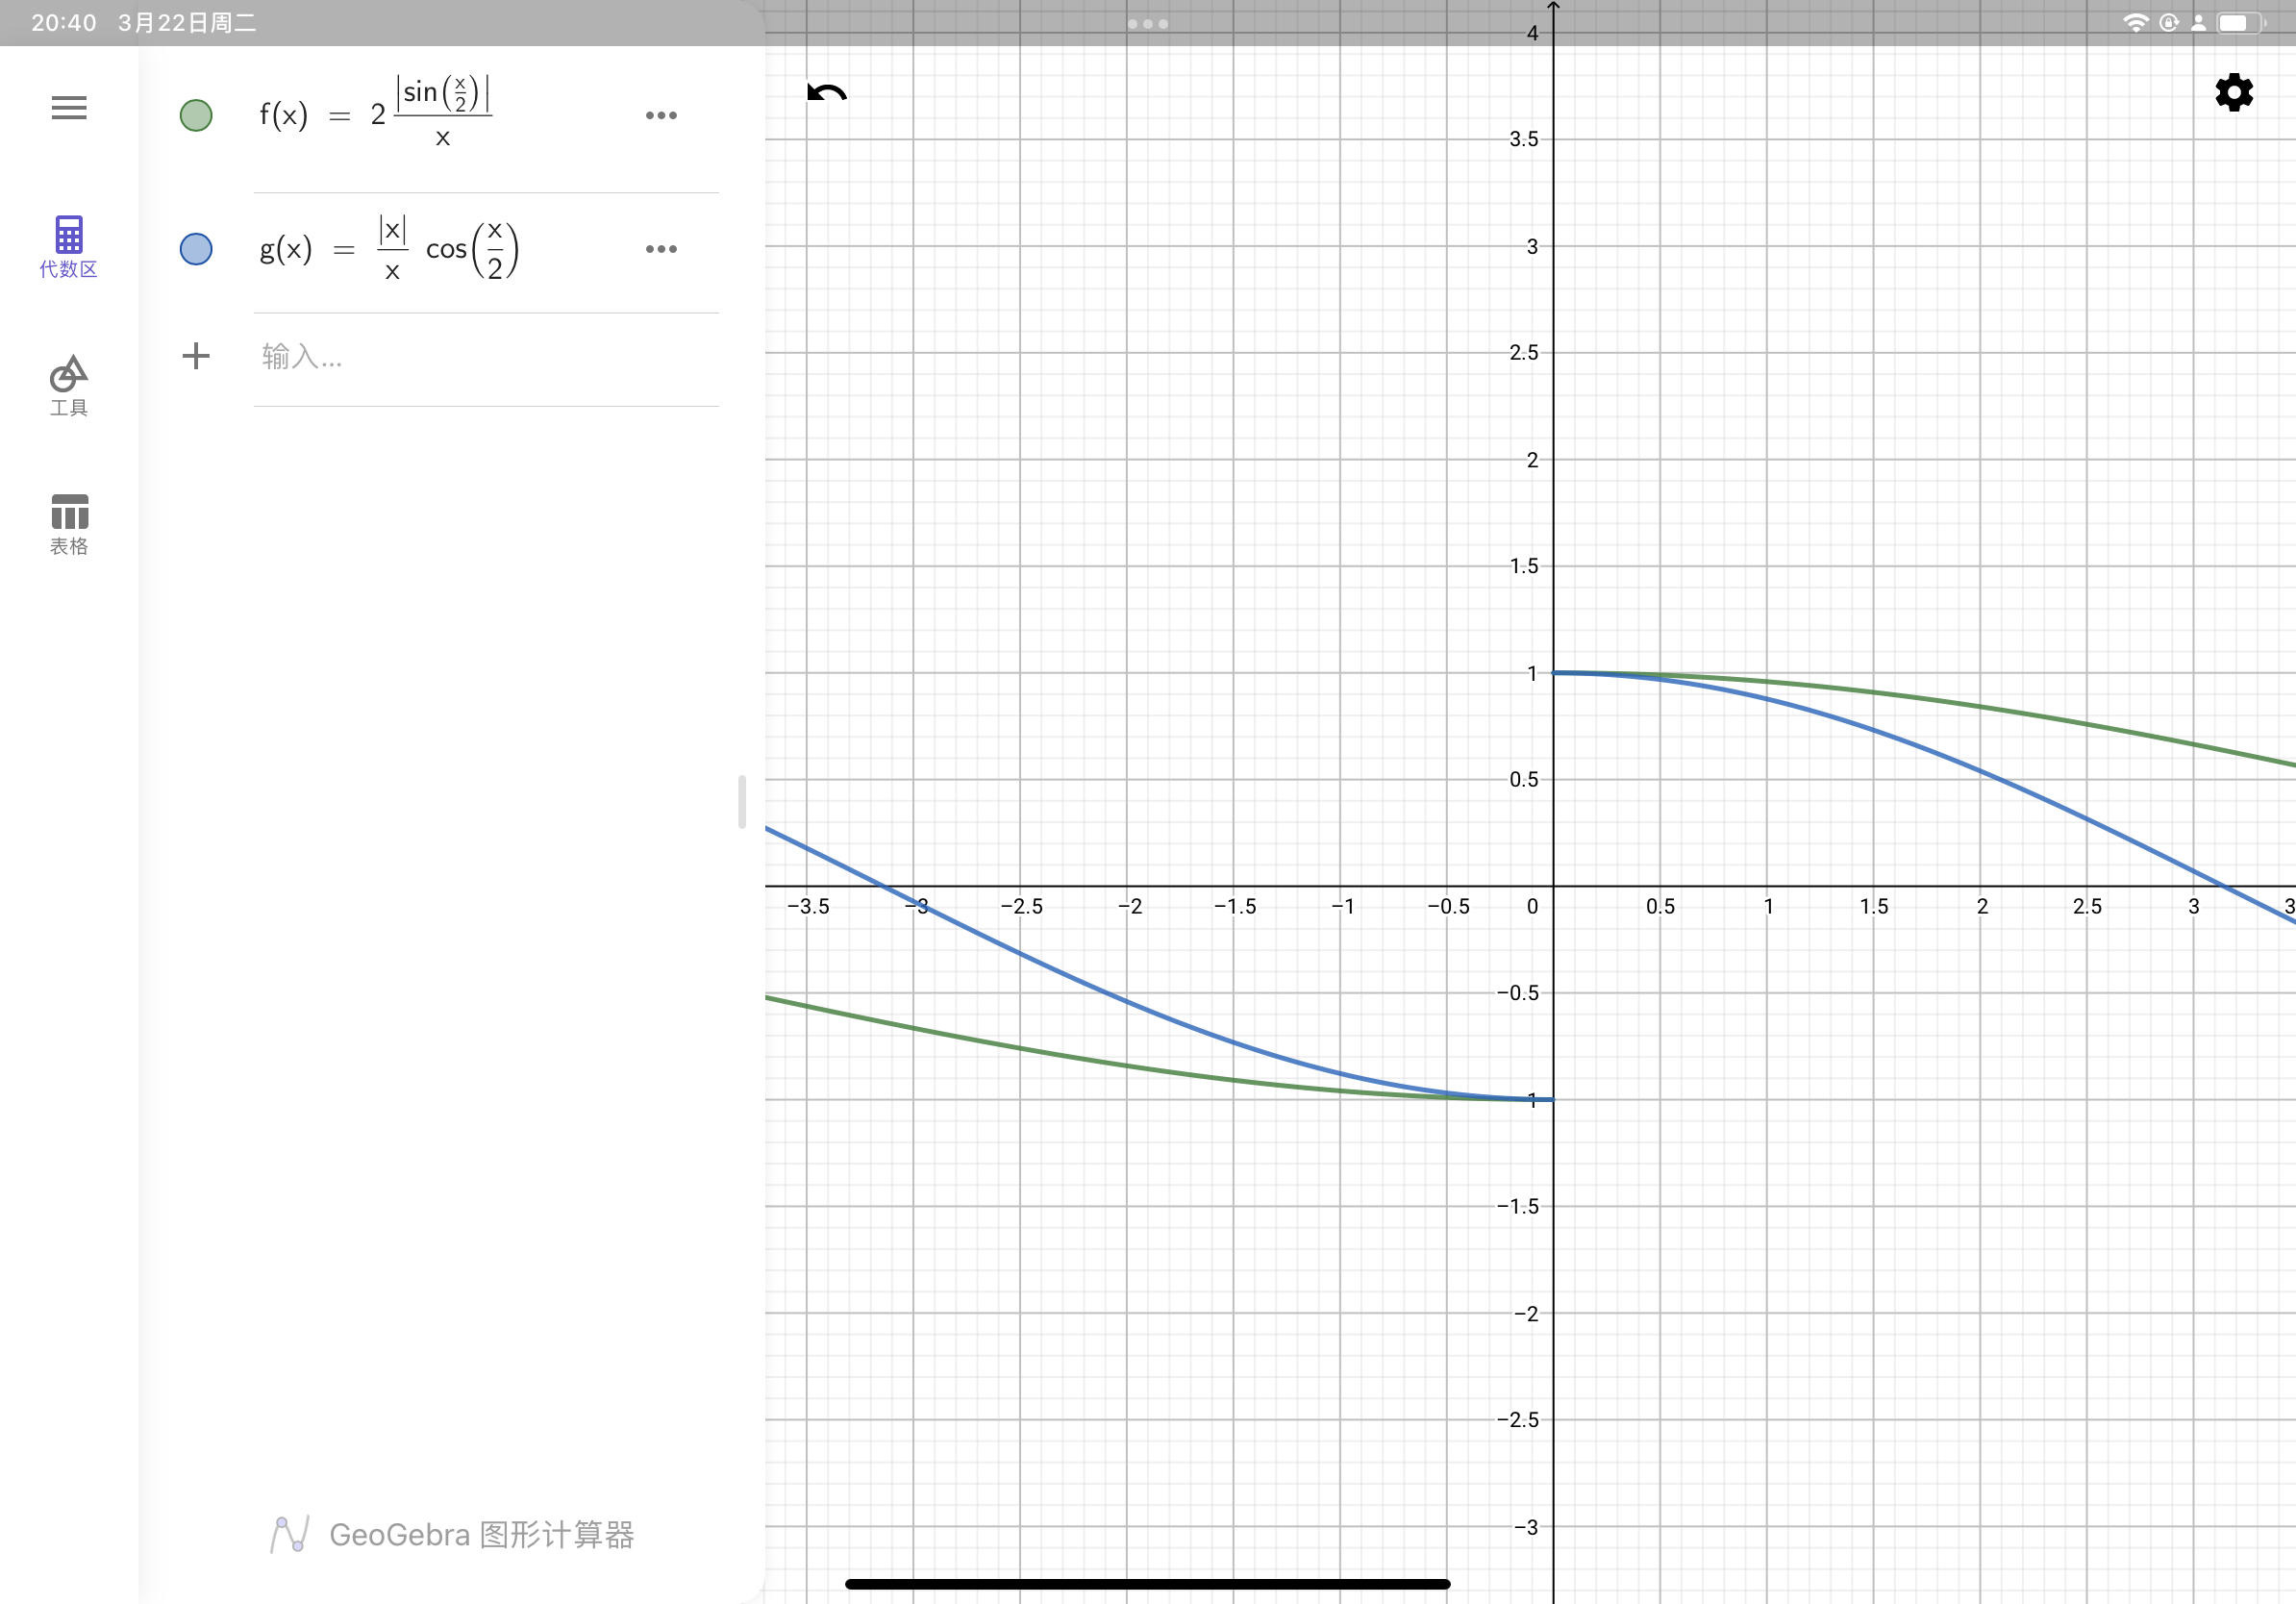
\includegraphics[scale=0.32]{9-2.png}
	\end{center}
	其中蓝线为群速度,绿线为相速度。 \\
	当波长很长时,有:
	\[
		\omega \approx a\sqrt{\frac{\kappa}{m}}k.
	\]
	则声速为:
	\[
		v_{sound} = a\sqrt{\frac{\kappa}{m}}.
	\]
	密度为:$\rho = \frac{m}{a}$,压缩系数倒数为:$\frac{1}{\beta} = -L\frac{dF}{dL} = -Na\frac{dF}{N\,da} = -a\kappa$。则有:
	\[
		v_{sound} = \sqrt{a}{m}\sqrt{a\kappa} = \frac{1}{\sqrt{\rho\beta}}.
	\]
	\end{tcolorbox}
	
	\item Find the expression for $g(\omega)$, the density of states of modes per angular frequency. \\
	$\triangleright$ Sketch $g(\omega)$.
	\begin{tcolorbox}[breakable, colback = black!5!white, colframe = black]
	态密度为:
	\[
		g(\omega) = \frac{\partial N}{\partial \omega} = 2\frac{\partial N}{\partial k}\frac{\partial k}{\partial \omega} = \frac{2}{v_g}\frac{\partial N}{\partial k}.
	\]
	上式中2是因为一个$\omega$对应两个波矢量$k$。由于在k空间中态均匀分布,则有:
	\[
		\frac{\partial N}{\partial k} = \frac{N}{k} = \frac{Na}{2\pi}.
	\]
	则态密度为:
	\[
		g(\omega) = \frac{Na}{\pi v_g} = \frac{N}{\pi}\sqrt{\frac{m}{\kappa}} \frac{\vert k \vert}{k}\frac{1}{\cos(ka/2)}.
	\]
	在$0\leq k \leq \frac{\pi}{a}$区域内,有:
	\[
		g(\omega) = \frac{N}{\pi}\frac{1}{\sqrt{(\kappa/m) - (\omega/2)^2}}.
	\]
	绘图如下:
	\begin{center}
		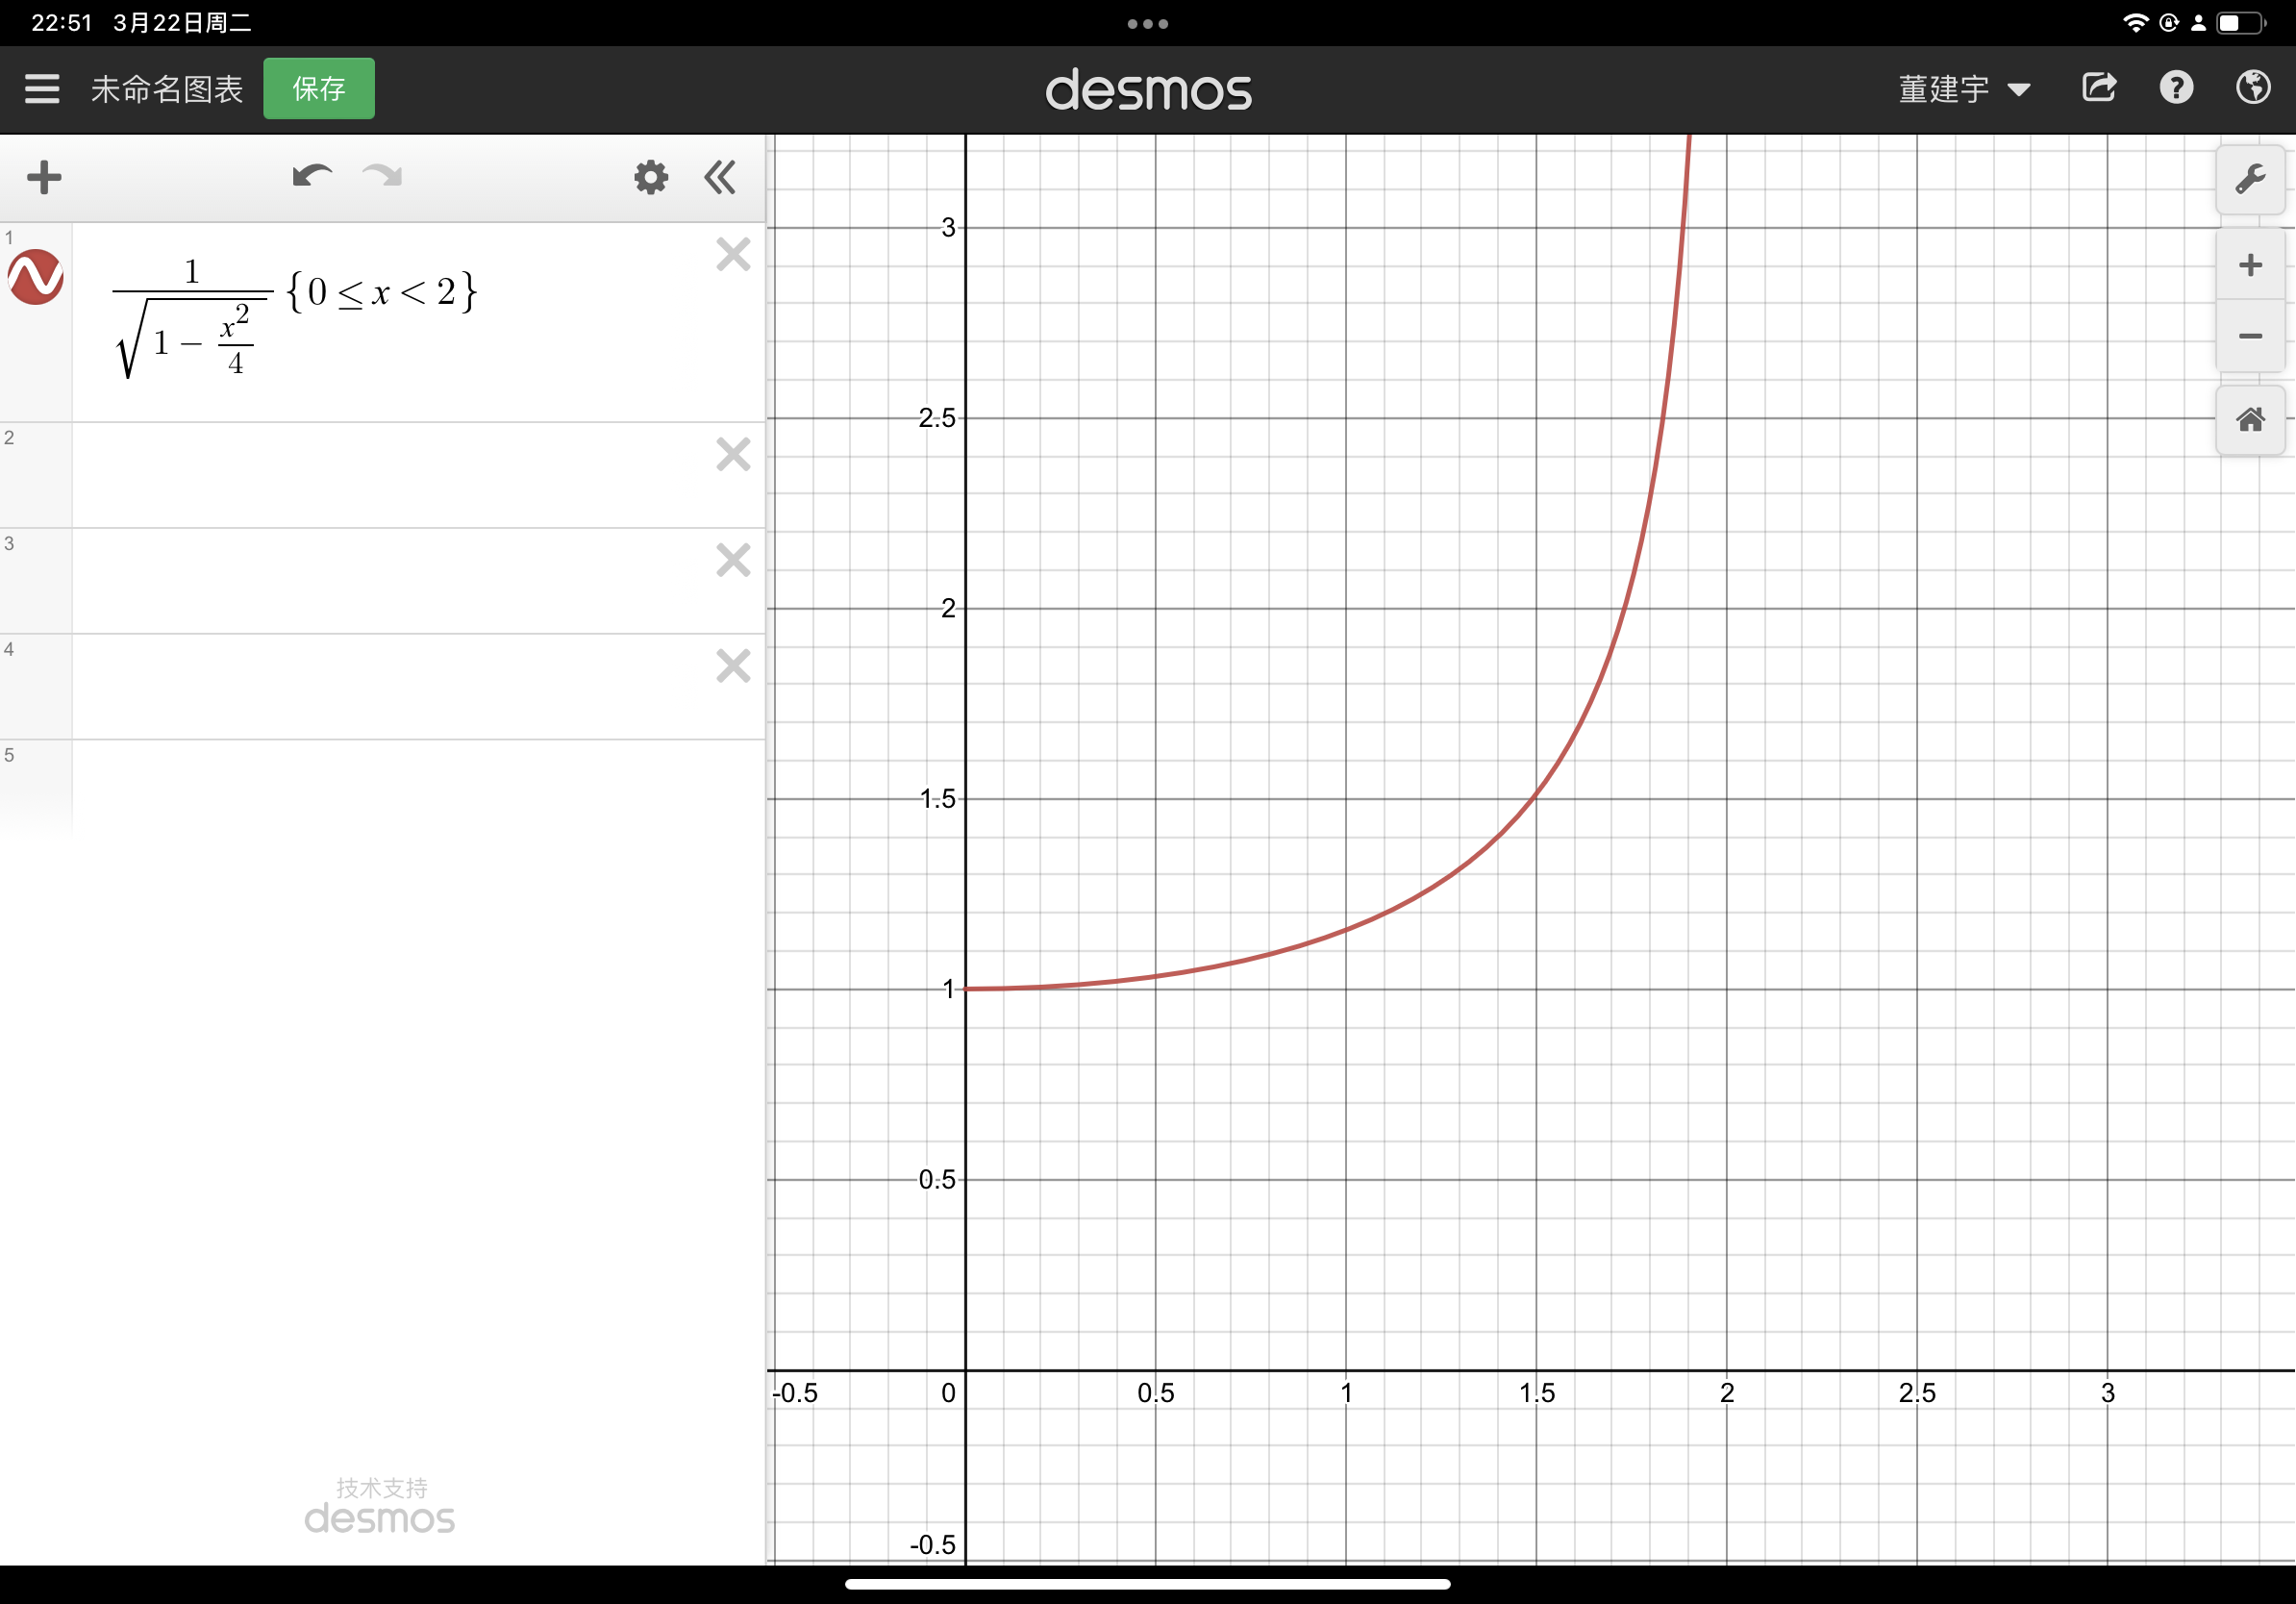
\includegraphics[scale = 0.32]{9-2-e.png}
	\end{center}
	纵坐标量纲与$N/(\pi \sqrt{\kappa/m})$相同;横坐标量纲与$\sqrt{\kappa/m}$相同。
	\end{tcolorbox}
	
	\item Write and expression for the heat capacity of this one-dimensional chain. You will inevitably have an integral that you cannot do analytically. 
	\begin{tcolorbox}[breakable, colback = black!5!white, colframe = black]
	内能为:
	\[
		U = \int_0^{\omega_{max}} \,d\omega g(\omega) \hbar\omega \left(\frac{1}{e^{\beta\hbar\omega}-1} + \frac{1}{2}\right) = \int_0^{\omega_{max}} \,d\omega \frac{N}{\pi} \frac{\hbar\omega}{\sqrt{(\kappa/m) - (\omega/2)^2}} \left(\frac{1}{e^{\beta\hbar\omega}-1} + \frac{1}{2}\right)
	\]
	其中$\beta = \frac{1}{kT}$,$\omega_{max} = 2\sqrt{\frac{\kappa}{m}}$。热熔为:
	\[
		C = \frac{\partial U}{\partial T} = \int_0^{\omega_{max}} \frac{N}{\pi} \frac{\hbar\omega}{\sqrt{(\kappa/m) - (\omega/2)^2}} \frac{e^{\beta\hbar\omega}}{(e^{\beta\hbar\omega} -1)^2} \frac{\hbar\omega}{k T^2}.
	\]
	\end{tcolorbox}
	
	\item However, you can expand exponentials for high temperature to obtain a high-temperature approximation. It should be obvious that the high-temperature limit should give heat capacity $C/N = k_B$ (the law of Dulong-Petit in one dimension). By expanding to next non-trivial order, show that 
	\[
		C/N = k_B(1-A/T^2+ \cdots)
	\]
	where
	\[
		A = \frac{\hbar^2\kappa}{6mk_B^2}.
	\]\begin{tcolorbox}[breakable, colback = black!5!white, colframe = black]
	在高温极限下,有$\beta \to 0$,$x = \beta\hbar\omega \to 0$,则有:
	\[
		%\frac{1}{e^x-1} = \frac{e^{-x}}{1-e^{-x}} = \sum_{l=1}^{+\infty} e^{-lx}.
		\frac{x}{e^x-1} = 1 - \frac{x}{2} + \frac{x^2}{12} + \mathcal{O}(x^2).
	\]
	则有:
	\[
		\frac{1}{e^{\beta\hbar\omega}-1} = \frac{kT}{\hbar\omega} - \frac{1}{2} + \frac{\hbar\omega}{12kT}.
	\]
	则内能为:
	\[
		E = \int_0^{\omega_{max}} \,d\omega \frac{N}{\pi} \frac{\hbar\omega}{\sqrt{(\kappa/m) - (\omega/2)^2}} \left( \frac{kT}{\hbar\omega} + \frac{\hbar\omega}{12kT} \right).
	\]
	热熔为:
	\[
		C = \frac{\partial E}{\partial T} = \int_0^{\omega_{max}} \,d\omega \frac{N}{\pi} \frac{\hbar\omega}{\sqrt{(\kappa/m) - (\omega/2)^2}} \left( \frac{k}{\hbar\omega} - \frac{\hbar\omega}{12kT^2} \right).
	\]
	可以计算得:
	\[
		\int_0^{\omega_{max}} \,d\omega \frac{N}{\pi} \frac{\hbar\omega}{\sqrt{(\kappa/m) - (\omega/2)^2}} \frac{k}{\hbar\omega} = k\int_0^{\omega_{max}} g(\omega) \,d\omega = kN.
	\]
	\[
		\int_0^{\omega_{max}} \,d\omega \frac{N}{\pi} \frac{\hbar\omega}{\sqrt{(\kappa/m) - (\omega/2)^2}} \frac{\hbar\omega}{12kT^2} = \frac{N\hbar^2}{12\pi k T^2} \int_0^{\omega_{max}} \frac{\omega^2}{\sqrt{(\kappa/m) - (\omega/2)^2}}\,d\omega.
	\]
	令$x = \frac{\omega}{\omega_{max}}$,则积分化为:
	\[
		\frac{\omega_{max}^3}{\sqrt{\kappa/m}}\int_0^1 \frac{x^2}{\sqrt{1-x^2}}\,dx = 2\pi\frac{\kappa}{m}.
	\]
	则热熔为:
	\[
		C = kN - \frac{N\hbar^2\kappa}{6mkT^2} = kN \left( 1 - \frac{\hbar^2\kappa}{6k^2m} \frac{1}{T^2} \right).
	\]
	即
	\[
		\frac{C}{N} = k_B (1-A/T^2 + \cdots)
	\]
	其中
	\[
		A = \frac{\hbar^2\kappa}{6mk_B^2}.
	\]
	\end{tcolorbox}
	
\end{enumerate}

\section{\textbf{(9.4) Decaying Waves}}
In the dispersion curve of the harmonic chain (Eq. 9.3), there is a maximum possible frequency of oscillation $\omega_{max}$. If a vibration with frequency $\omega > \omega_{max}$ is forced upon the chain (say by a driving force) the "wave" will not propagate along the chain, but rather will decay as one moves away from the point where the oscillation is imposed (this is sometimes known as an "evanescent" wave). With $\omega>\omega_{max}$ solve Eq. 9.3 for a complex $k$ to determine the decay length of this evanescent wave. What happens to this length as $\omega \to \omega_{max}$?
\begin{tcolorbox}[breakable, colback = black!5!white, colframe = black]
如果一个频率$\omega>\omega_{max}$的驱动力加在一位原子链上,则波矢量$k$为一个复数。则有:
\[
	\sin\left( \frac{ka}{2} \right) = \frac{1}{2i} \left( e^{ika/2} - e^{-ika/2} \right).
\]
方程9.3可以写为:
\[
	\sin\left( \frac{ka}{2} \right) = \frac{1}{2i} \left( e^{ika/2} - e^{-ika/2} \right) = \pm\frac{\omega}{2}\sqrt{\frac{m}{k}}.
\]
令$x = \frac{ka}{2}$,$y = \frac{\omega}{2}\sqrt{\frac{m}{\kappa}}$,则有:
\[
	e^{2ix} \mp 2iye^{ix} - 1 = 0.
\]
则有:
\[
	e^{ix} = \pm iy \pm \sqrt{1-y^2}
\]
当$\omega > \omega_{max} = 2\sqrt{\frac{\kappa}{m}}$时,$y = \frac{\omega}{\omega_{max}} > 1$。令$k = k_0+ik_1$,其中$k_0$,$k_1$都为实数。则上述方程为:
\[
	e^{-k_1a/2} e^{ik_0a/2} = \pm i\left( \frac{\omega}{\omega_{max}} +\sqrt{\frac{\omega^2}{\omega_{max}^2} - 1} \right).
\]
两侧实部虚部对应相等,有
\begin{align*}
	e^{-k_1a/2}\cos(k_0a/2) &= 0 \\
	e^{-k_1a/2}\sin(k_0a/2) &= \pm \left( \frac{\omega}{\omega_{max}} +\sqrt{\frac{\omega^2}{\omega_{max}^2} - 1} \right).
\end{align*}
则有:
\[
	k_0 = \mp \frac{\pi}{a}; ~~ k_1 = \frac{2}{a}\ln \left( \frac{\omega}{\omega_{max}} +\sqrt{\frac{\omega^2}{\omega_{max}^2} - 1} \right).
\]
则衰减长度为:
\[
	d = \frac{1}{k_1} = \frac{a}{2}\frac{1}{\ln \left( \frac{\omega}{\omega_{max}} +\sqrt{\frac{\omega^2}{\omega_{max}^2} - 1} \right)}。
\]
当$\omega \to \omega_{max}$时,
\[
	d \to \frac{a}{2} \frac{1}{\ln1} \to \infty.
\]
\end{tcolorbox}

\end{document}